\documentclass[tikz,border=10pt]{standalone}
\usetikzlibrary{shapes.multipart,positioning,arrows.meta}

\begin{document}

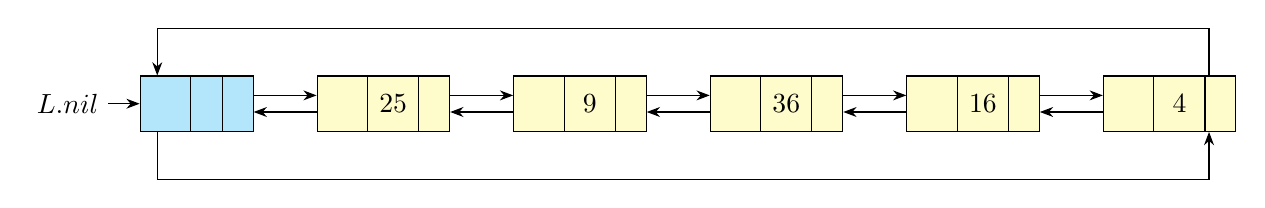
\begin{tikzpicture}[
>=Stealth,
node distance=.8cm,
node/.style={
rectangle split,
rectangle split parts=3,
rectangle split horizontal,
draw,
minimum height=2em,
text width=.4cm,
align=center},
normal/.style={node,fill=yellow!20},
active/.style={node,fill=cyan!30}
]

\node[active] (n0) {};
\node[left=.4cm of n0] (L) {$L.nil$};
\draw[->] (L)--(n0);

\foreach \v[count=\i,remember=\i as \p(initially 0)] in {25,9,36,16,4}{
\node[normal,right=of n\p] (n\i) {\nodepart{two}\v};
\draw[->] ([yshift=3pt]n\p.east)--([yshift=3pt]n\i.west);
\draw[->] ([yshift=-3pt]n\i.west)--([yshift=-3pt]n\p.east);
}

\draw[->] ([xshift=.5cm]n5.north)--++(0,.6)-|([xshift=-.5cm]n0.north);
\draw[->] ([xshift=-.5cm]n0.south)--++(0,-.6)-|([xshift=.5cm]n5.south);

\end{tikzpicture}

\end{document}
